\begin{figure*}
  \centering
  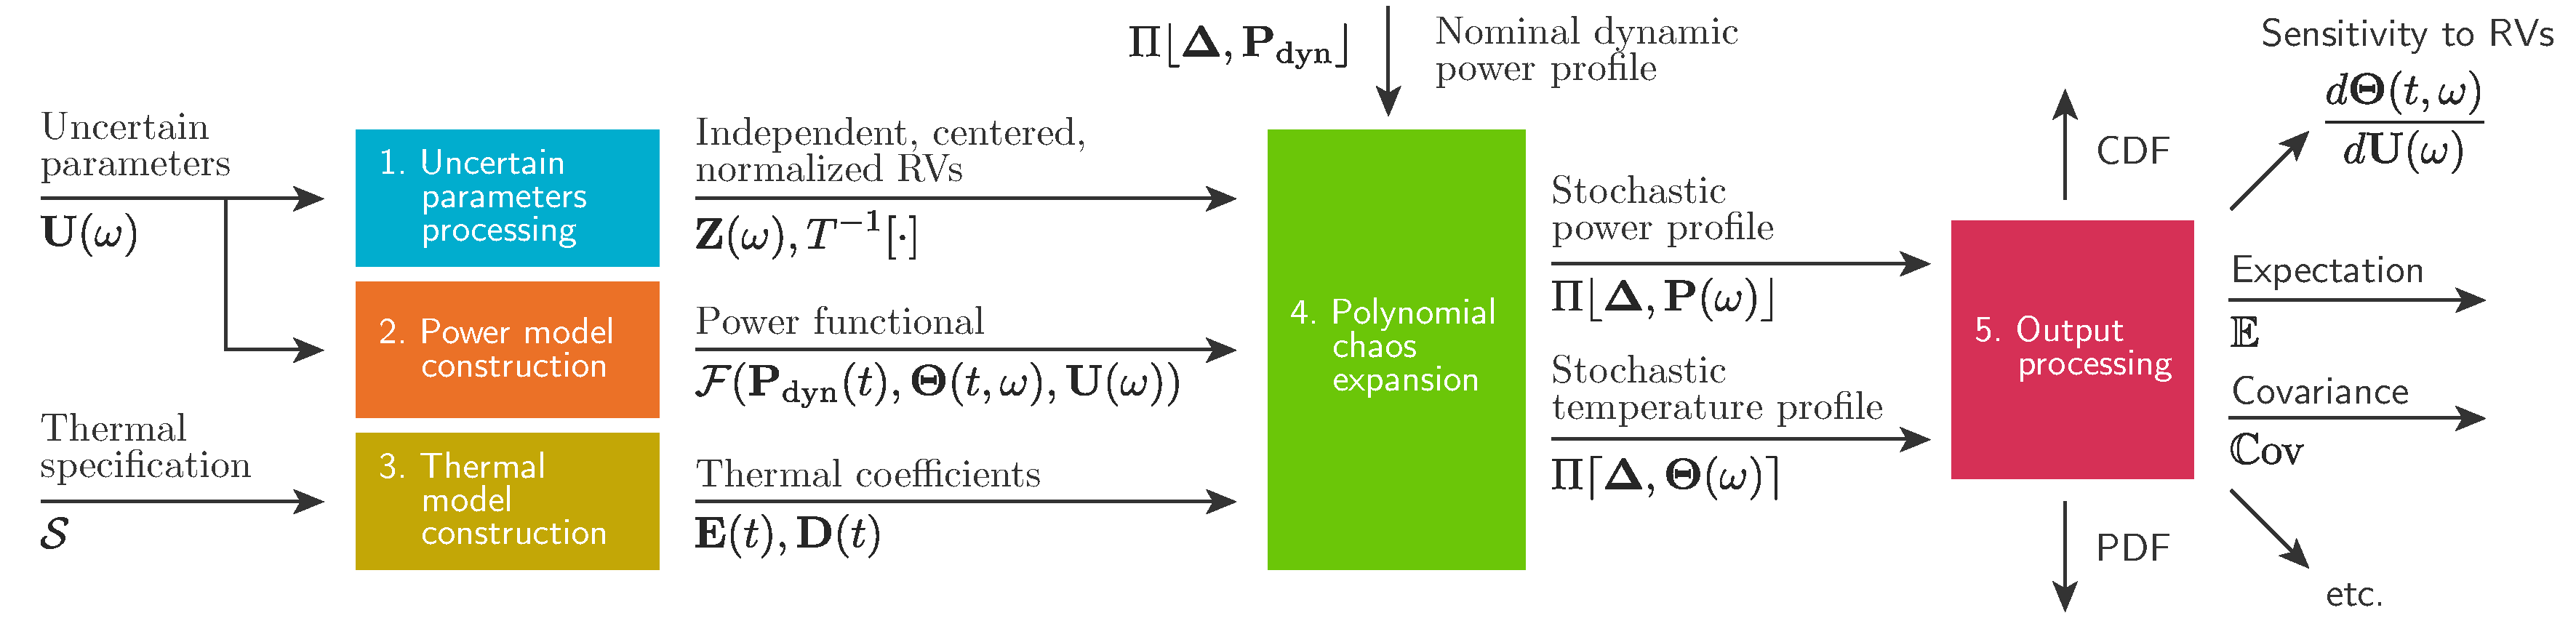
\includegraphics[width=0.9\textwidth]{include/assets/algorithm.pdf}
  \vspace{-0.7em}
  \caption{The structure of the proposed framework.}
  \flabel{algorithm}
  \vspace{-1.6em}
\end{figure*}

Consider a heterogeneous electronic system that consists of $\nprocs$ processing
elements and is equipped with a thermal package. A (transient) power profile
$\profileP$ is defined as a tuple composed of a data matrix $\mP \in
\real^{\nprocs \times \nsteps}$ that captures the power dissipation of the
$\nprocs$ processing elements at $\nsteps$ moments of time and a (column) vector
$\partition{\mP} = (\t_i) \in \real^{\nsteps}$ with positive and strictly
increasing components that specifies these moments of time. The definition of a
(transient) temperature profile $\profileT$ is the same as the one for power
except that the data matrix $\mTO$ contains temperature values.

The system depends on a set of process parameters that are uncertain at the
design stage. These parameters are denoted by a random vector $\vU \in
\real^\nparams$. This dependency leads to deviations of the actual power
dissipation from the nominal values and, therefore, to deviations of temperature
from the one corresponding to the nominal power consumption.

The goal of this work is to develop a system-level probabilistic framework for
transient power-temperature analysis (PTA) of electronic systems where the
actual power dissipation and temperature are stochastic due to their dependency
on the uncertain parameters $\vU$. The user is required to: (a) provide a
thermal specification of the platform, denoted by $\system$; (b) have prior
knowledge (or belief) about the probability distribution of the uncertain
parameters; and (c) specify a power model, in which $\vU$ is an input. The
framework should provide the user with the tools to analyze the system under a
given workload, without imposing any constraints on the nature/origins of this
workload, and obtain the corresponding stochastic power $\profileP$ and
temperature $\profileT$ profiles with a desired level of accuracy and at low
costs.
